\documentclass{beamer} %[12pt,handout]

\usepackage[english]{babel}
\selectlanguage{english}
\usepackage[utf8]{inputenc}
\usepackage{hyperref}
\usepackage{url}
\usepackage{csvsimple}
\usepackage{bera}% optional: just to have a nice mono-spaced font
\usepackage{listings}
\usepackage{xcolor}
\usepackage{graphicx}
\usepackage{listings}

\colorlet{punct}{red!60!black}
\definecolor{background}{HTML}{EEEEEE}
\definecolor{delim}{RGB}{20,105,176}
\colorlet{numb}{magenta!60!black}

\lstset{basicstyle=\ttfamily,
  showstringspaces=false,
  commentstyle=\color{red},
  keywordstyle=\color{blue},
  breaklines=true,
  postbreak=\raisebox{0ex}[0ex][0ex]{\ensuremath{\color{black}\hookrightarrow\space}},
  morekeywords={run, p, e, v, name,d, FROM, MAINTAINER, LABEL, ENV, RUN, ADD, EXPOSE, ENV, VOLUME, WORKDIR, CMD, up, link, build,volumes_from, ports, volumes, links, image},
  xleftmargin=-30pt,
  xrightmargin=0pt,
}

\lstdefinelanguage{json}{
    basicstyle=\normalfont\ttfamily,
    numbers=left,
    numberstyle=\scriptsize,
    stepnumber=1,
    numbersep=8pt,
    showstringspaces=false,
    breaklines=true,
    frame=lines,
    backgroundcolor=\color{background},
    literate=
     *{0}{{{\color{numb}0}}}{1}
      {1}{{{\color{numb}1}}}{1}
      {2}{{{\color{numb}2}}}{1}
      {3}{{{\color{numb}3}}}{1}
      {4}{{{\color{numb}4}}}{1}
      {5}{{{\color{numb}5}}}{1}
      {6}{{{\color{numb}6}}}{1}
      {7}{{{\color{numb}7}}}{1}
      {8}{{{\color{numb}8}}}{1}
      {9}{{{\color{numb}9}}}{1}
      {:}{{{\color{punct}{:}}}}{1}
      {,}{{{\color{punct}{,}}}}{1}
      {\{}{{{\color{delim}{\{}}}}{1}
      {\}}{{{\color{delim}{\}}}}}{1}
      {[}{{{\color{delim}{[}}}}{1}
      {]}{{{\color{delim}{]}}}}{1},
}

  \hypersetup{
    pdfauthor={Georges Alkhouri, Tom Neumann},
    pdftitle={Final Presentation - Dockerizing Linked Data}
  }

\usetheme{default}
\setbeamercolor{title}{fg=black}
\setbeamercolor{frametitle}{fg=black}
\setbeamercolor{description item}{fg=black}
\setbeamercolor{enumerate item}{fg=black}
\setbeamercolor{itemize item}{fg=black}
\setbeamercolor{bibliography entry author}{fg=black}
\setbeamercolor{bibliography entry title}{fg=black}
\setbeamercolor{bibliography entry location}{fg=black}
\setbeamercolor{bibliography item}{fg=black}
\setbeamercolor{caption name}{fg=black}

\setbeamertemplate{itemize items}[circle]
%\setbeamertemplate{caption}{
%\begin{beamercolorbox}[wd=.5\paperwidth, sep=.2ex]{block body}\insertcaption
%\end{beamercolorbox}
%}

\addtobeamertemplate{frametitle}{\vskip+5.0ex}

\beamertemplatenavigationsymbolsempty

\setbeamertemplate{footline}[frame number]

\begin{document}

\title{Final Presentation - Dockerizing Linked Data}
\author{Georges Alkhouri, Tom Neumann}
\institute{University of Applied Sciences Leipzig}
\date{6th Jul. 2015}

\frame{\titlepage}

\frame{

\frametitle{Problem}

Populare knowledge bases faceing \textbf{performence/availability} issues through \textbf{high request} rates
\vspace{\baselineskip}

\centerline{Solution $\downarrow$} 

\vspace{\baselineskip}
Run a local mirror of the knowledge base with a SPARQL endpoint
}

\frame{

\frametitle{New Problem}

To run and maintain a local knowledge base environment is a complex task requiring a lot of effort and is not suitable for domain admins who just want to use the SPARQL interface
\vspace{\baselineskip}

\centerline{New Solution $\downarrow$} 

\vspace{\baselineskip}

\centerline{\textbf{Dockerizing Linked Data}}
}

\frame {
\frametitle{Usage Example: Professorenkatalog}

The Catalogus Professorum Lipsiensium

\begin{itemize}

\item Knowledge base of professors at the Leipzig University
\item Includes records from 1409 to presence
\item Comprises over 14, 000 entities
\item Many interlinked connections in the LOD Cloud
\item Curated by \textbf{historical researchers} and \textbf{interested citizen scientists}

\end{itemize}
}

\frame {
\frametitle{Usage Example: Professorenkatalog}
\framesubtitle{Infrastructure}

Professorenkatalogs infrastructure consists of several web applications (Presentation, Storage, Backup, ... )

}

\frame{

\begin{figure}
	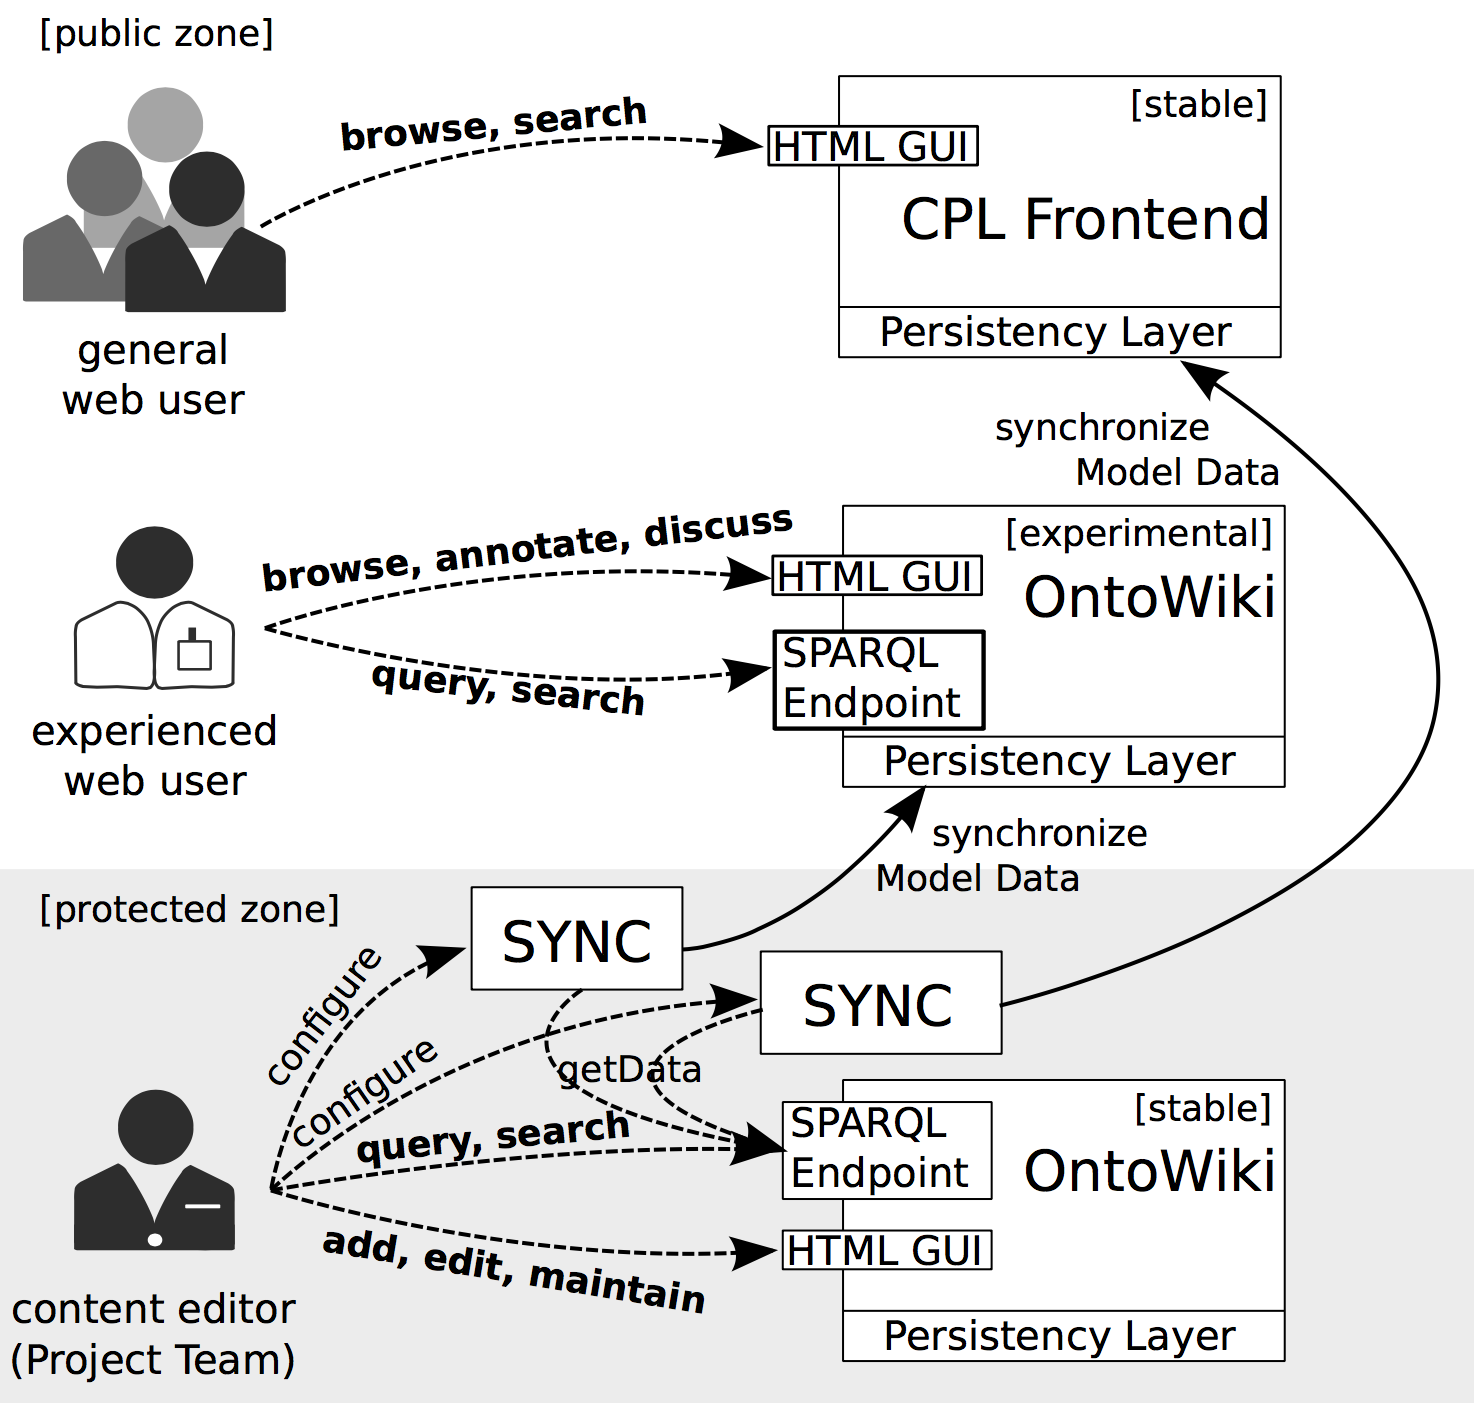
\includegraphics[scale=0.32]{CPL.png}
	\caption{Architecture of Professorenkatalog\cite[p. 6]{dld-paper}}
\end{figure}

}

\frame{
	\frametitle{What is Docker?}
	Docker is a free virtualisation technology, which is based on Linux Containers.
	\begin{figure}
		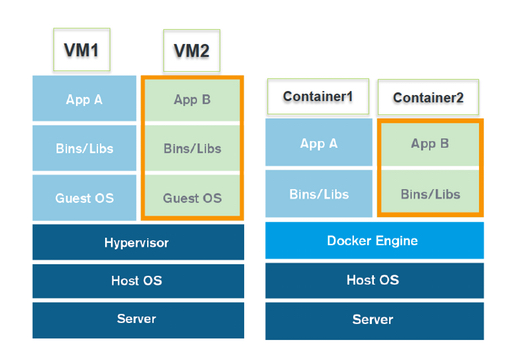
\includegraphics[scale=0.4]{vm-vs-docker.png}
		\caption{Virtual Machines vs Docker}
		%Quelle: : http://www.theregister.co.uk/2015/01/07/asigra_dockerises_cloud_backup/
	\end{figure}
}

\frame{
	\frametitle{What is Docker?}
	Introduction
	\begin{itemize}
		\item Docker consists of two components: \textbf{Docker Engine, Docker Hub}
		\item \textbf{Docker Engine} is managing the containers and deploys the applications on them 
		\item \textbf{Docker Hub} is a Docker repository to ship and run your applications anywhere
	\end{itemize}
}

\frame{
	\frametitle{What is Docker?}
	\framesubtitle{Docker's architecture}
	\begin{figure}
		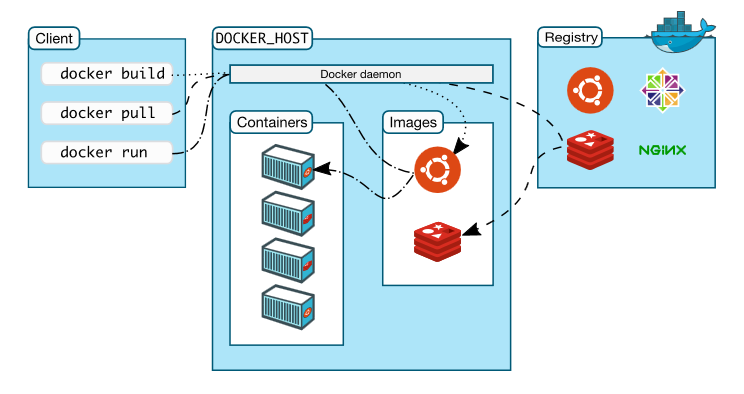
\includegraphics[scale=0.5]{docker-architecture.png}
		\caption{Architecture of Docker}
		%Quelle: : https://docs.docker.com/introduction/understanding-docker/
	\end{figure}
}

\frame{
	\frametitle{What is Docker?}
	\framesubtitle{Usage}
	\begin{enumerate}
		\item Install Docker.
		\item Pull (and modify) a Docker image from the Docker Hub or create a Dockerfile.
		\item Run a container by using the Docker image.
	\end{enumerate}
}

\setbeamercolor{description item}{fg=blue}
\setbeamercolor{itemize item}{fg=black}

\frame{
	\frametitle{What is Docker?}
	\framesubtitle{Basic commands}
	docker ...
	\begin{description}
	\item[build] \textit{dockerfile}: build an image from a Dockerfile
	\item[run] \textit{image}: run a command in a new container
	\item[start] \textit{name|id}: start a stopped container
	\item[stop] \textit{name|id}: stop a running container
	\item[rm] \textit{name|id}: remove a container
	\item[rmi] \textit{name|id}: remove an image
	\end{description}
}

\frame{
	\frametitle{Docker example: Virtuoso 7}
	Virtuoso is a SQL-ORDBMS and Web Application Server (Universal Server). The Server provides SQL, XML, RDF data mangement. Access to the Triple Store is available in many ways, for example via SPARQL, ODBC, JDBC. %(Quelle: https://www.w3.org/2001/sw/wiki/OpenLink_Virtuoso)
}

\setbeamertemplate{frametitle continuation}{}
\frame[allowframebreaks]{
	\frametitle{Docker example: Virtuoso 7}
	\begin{tiny}
	\begin{lstlisting}[caption=Vituoso 7 Dockerfile]
	FROM debian:jessie
	MAINTAINER Natanael Arndt ...
	ENV DEBIAN_FRONTEND noninteractive
	RUN apt-get update
	# install some basic packages
	RUN apt-get install -y libldap-2.4-2 libssl1.0.0 unixodbc
	ADD virtuoso-minimal_7.2_all.deb \
	virtuoso-opensource-7-bin_7.2_amd64.deb \
	libvirtodbc0_7.2_amd64.deb
	RUN dpkg -i virtuoso-minimal_7.2_all.deb \
	virtuoso-opensource-7-bin_7.2_amd64.deb \
	libvirtodbc0_7.2_amd64.deb
	ADD virtuoso.ini.dist /
	ADD run.sh /
	# expose the ODBC and management ports to the outer world
	EXPOSE 1111
	EXPOSE 8890
	ENV PWDDBA="dba"
	VOLUME "/var/lib/virtuoso/db"
	VOLUME "/import_store"
	WORKDIR /var/lib/virtuoso/db
	CMD ["/run.sh"] 
	\end{lstlisting}
	\end{tiny}	
}

\frame{

	\frametitle{Simple Docker Demo}
	\framesubtitle{Virtuoso Container}
	
	Dockerizing project is hosting an own virtuoso image at:
	
	\begin{center}
		\url{https://registry.hub.docker.com/u/aksw/dld-store-virtuoso7/}
	\end{center}
	
}

\setbeamertemplate{frametitle continuation}{}
\frame[allowframebreaks]{

	\frametitle{Simple Docker Demo}
	\framesubtitle{Run Container}

\begin{center}

	Start and run a docker container through:

	\begin{lstlisting}
	
	docker run -d 
	           --name="virtuoso" 
	           -p <host port>:8890 //SPARQL
	           -p <host port>:1111 //ODBC
                   -e PWDDBA="super secret" 
                   -v <host virtuoso directory>:/var/lib/virtuoso/db
                    aksw/dld-store-virtuoso7

	\end{lstlisting}

\end{center}
}

\frame{
	
	\frametitle{Simple Docker Demo}
	\framesubtitle{What is going on?}
	
	\begin{description}
	
	\item[run] Run a command in a new container
	\item[-d] Run container in background and print container ID
	\item[- -name] Assign a name to the container
	\item[-p] Publish a container's port to the host
	\item[-e] Set environment variables into container
	\item[-v] Bind mount a volume
	
	\end{description}
	
	"aksw/dld-store-virtuoso7" is the image name, local or on docker hub

}

\frame{

	\frametitle{Simple Docker Demo}
	\framesubtitle{Setup Virtuoso}

	The virtuoso.ini file is injected into the container through \colorbox{background}{\lstinline{-v}} which mounts the datebase folder from the host system into the container
	\vspace{\baselineskip}
	
	If not specified the container provides a fallback file

}


\frame{

	\frametitle{Simple Docker Demo}
	\framesubtitle{Access Virtuoso Container}

	After \colorbox{background}{\lstinline{docker run}} docker provides an access to the container through the exposed port (\colorbox{background}{\lstinline{-p 8890:8890}}) on localhost
	
	\begin{center}
		\url{http://localhost:8890/sparql}
	\end{center}

}

\frame{

	\begin{figure}
	
	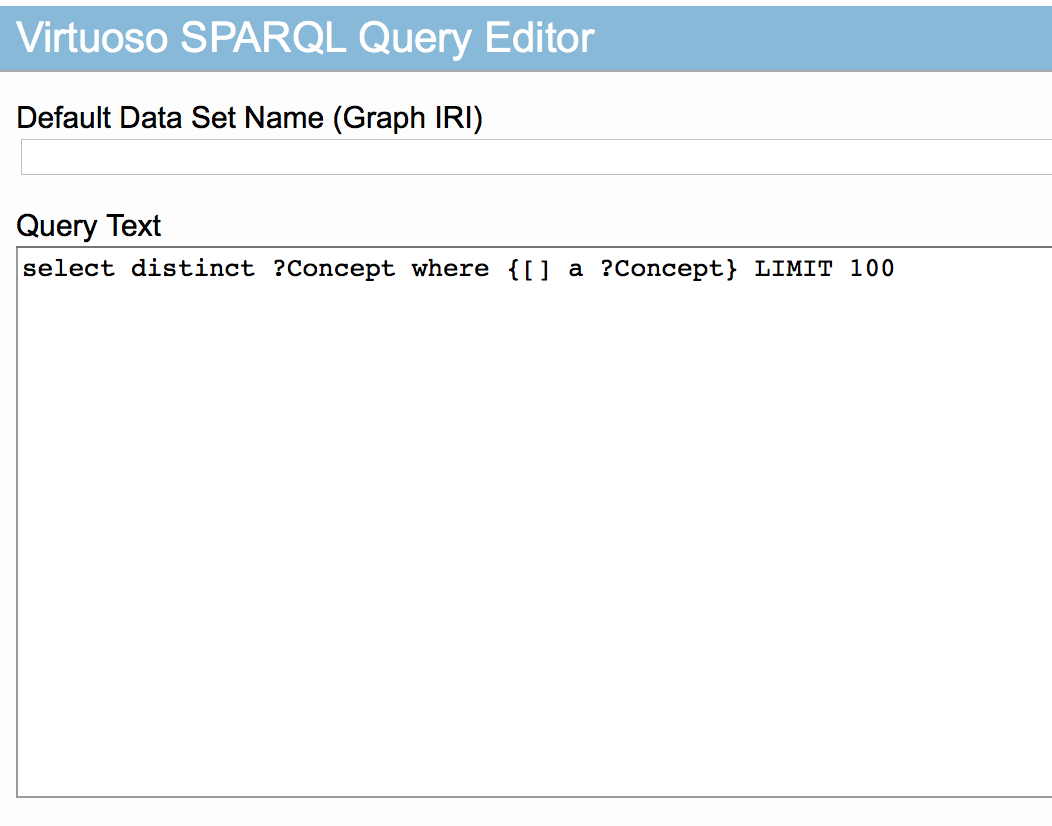
\includegraphics[scale=0.25]{virtuoso-sparql.png}
	\caption{Virtuoso SPARQL Endpoint provided by a docker container}
	
	\end{figure}
}

\frame{
	\frametitle{Multiple Containers}
	\framesubtitle{Communication}

	\begin{center}
	
	Containers can connect and expose information with each other
	
	\end{center}

}

\frame{
	\frametitle{Multiple Containers}
	\framesubtitle{Communication Approaches}
	
	\textbf{Network port mapping}
	\begin{itemize}
	
	\item[] Maps a port inside the container to a port on the host (\colorbox{background}{\lstinline{docker run ... -p 8890:8890 ...}})
	
	\end{itemize}
	
	\textbf{Linking System}
	\begin{itemize}
	
	\item[] Source containers information can be sent to a recipient container by naming the source 
	\item[] \colorbox{background}{\lstinline{docker run --name="db" ...}}
	\item[] and linking it to a recipient
	\item[] \colorbox{background}{\lstinline{docker run --link="db" ...  webserver}}
	\end{itemize}
}

\frame{
	\frametitle{Multiple Containers}
	\framesubtitle{Linking System - Shared Information}
	
	\textbf{Environment variables}
	\begin{itemize}
		\item[] Docker creates Environment variables in target container
		\begin{itemize}
			\item[] ...
			\item[] DB\_NAME=db
			\item[] DB\_PORT=tcp://172.17.0.5:5432
			\item[] DB\_PORT\_5432\_TCP=tcp://172.17.0.5:5432
			\item[] DB\_PORT\_5432\_PROTO=tcp
			\item[] DB\_PORT\_5432\_PORT=5432
			\item[] DB\_PORT\_5432\_ADDR=172.17.0.5
			\item[] ...
		\end{itemize} 
	\end{itemize}
	
}

\frame{
	\frametitle{Multiple Containers}
	\framesubtitle{Linking System - Shared Information}
	
	\textbf{Updating the /etc/hosts file}
	\begin{itemize}
		\item[] Docker adds a host entry for the source container
		\item[] Automatically updates  hosts file with new IP when source container restarts
	\end{itemize}
}


\frame{

	\frametitle{Dockerizing Linked Data}
	
	The Project wants to improve the setup of linked data environments and make the replacement of components more easier 
	\vspace{\baselineskip}
	
	\centerline{through $\downarrow$} 
	\vspace{\baselineskip}

	\centering{Applying \textbf{micro service architecture} with Docker}

}

\frame{

	\frametitle{Dockerizing Linked Data}
	\framesubtitle{Containerised Knowledge Base}
	
	\begin{figure}
	
	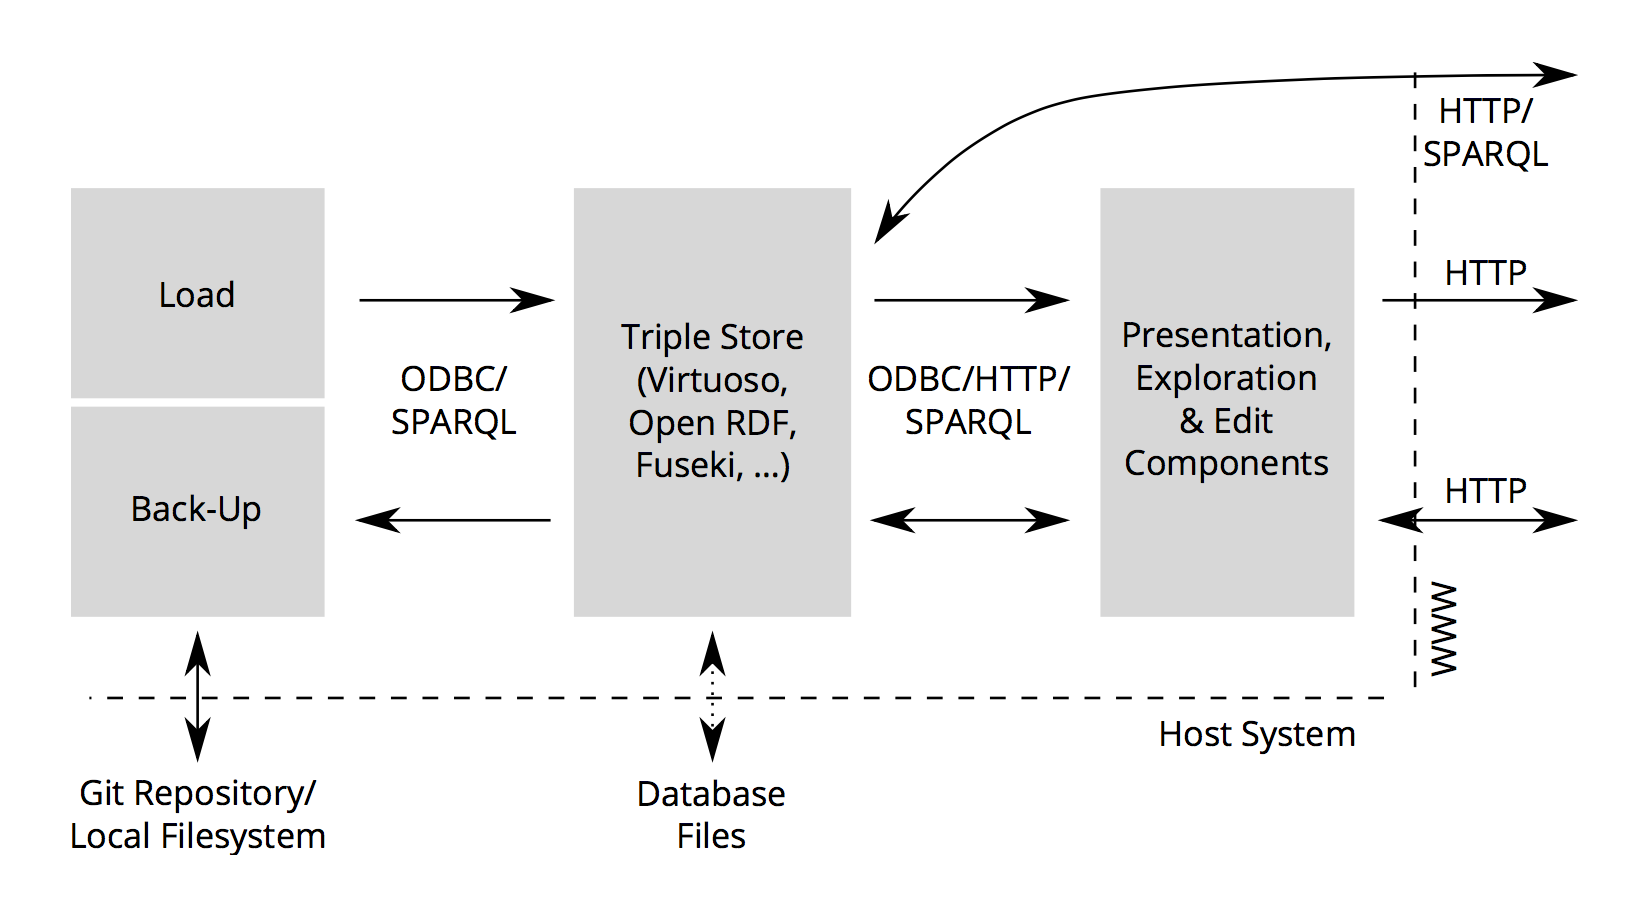
\includegraphics[scale=0.33]{dockerizing-container.png}
	\caption{Architecture and data-flow of the containerized micro services\cite[p. 3]{dld-paper}}
	
	\end{figure}
}

\frame{

	\frametitle{Dockerizing Linked Data}
	\framesubtitle{Docker Compose}
	
	The Dockerizing application works with Docker Compose
	\vspace{\baselineskip}
		
	Docker Compose:
	
	\begin{itemize}
  		\item Tool for defining and running \textbf{multi-container} applications
		\item Define a multi-container application in a single file
	\end{itemize}
	
}

\frame{

	\frametitle{Dockerizing Linked Data}
	\framesubtitle{Docker Compose how it works}
	
	\begin{enumerate}
	
		\item Write some Dockerfiles for reproducing your images
		\item Define the services that make up your app in \textbf{docker-compose.yml}
		\item Run \colorbox{background}{\lstinline{docker-compose up}} and Compose will start and run all services
	
	\end{enumerate}
	
}

\frame[allowframebreaks]{

	\frametitle{Dockerizing Linked Data}
	\framesubtitle{docker-compose.yml file}
	
	\begin{small}
	\begin{lstlisting}[caption=Compose file example from Docker]
		web:
 		    build: .
  		    ports:
   			- "5000:5000"
  		    volumes:
  		    	- .:/code
  		    links:
   		   	- redis
		redis:
 		    image: redis
	\end{lstlisting}
	\end{small}
}

\frame[allowframebreaks]{

	\frametitle{Dockerizing Linked Data}
	
	Previous example is equal to following docker commands:
	\vspace{\baselineskip}

	\begin{small}
	\begin{lstlisting}
		docker run --name="redis" redis
		
		docker build -t web .
		docker run --link="redis" -p 5000:5000 -v .:/code --name="web" web
	\end{lstlisting}
	\end{small}	
}

\frame{

	\frametitle{Dockerizing Linked Data}
	\framesubtitle{Linking}
	
	Compose connects containers and shares volumes, IP adresses or environment variables to multiple containers with the \colorbox{background}{\lstinline{link}} or \colorbox{background}{\lstinline{volumes_from}} tag
}

\frame{
	\frametitle{Demo Dockerizing}
	\framesubtitle{Services}
	There are 4 kinds of services in the setup area of Dockerizing composer files:
	\newline
	\textbf{store} 
	\begin{itemize}
		\item the store service defines a Triple Store
		\item needs an image (e.g. aksw/dld-store-virtuoso7)
		\item needs a volume for persistent data storage
	\end{itemize}
	\textbf{load}
	\begin{itemize}
		\item the load service defines a load image (e.g. aksw/dld-load-virtuosoload)
		\item it is needed to load data into the store
	\end{itemize}	
}

\frame{
	\frametitle{Demo Dockerizing}
	\framesubtitle{Services}
	\textbf{backup}
	\begin{itemize}
		\item defines a backup component (e.g. aksw/dld-backup-virtuoso)
		\item this component should be used for a backup of the Triple Store data 
	\end{itemize}
	\textbf{present}
	\begin{itemize}
		\item defines one or more presentation images (e.g. aksw/dld-present-ontowiki)
		\item the component is used to explore the Triple Store data
	\end{itemize}
}

\frame{
	\frametitle{Summary}
	
}

\frame {
	\frametitle{References}

\begin{thebibliography}{Knowledge Base Shipping to the Linked Open Data Cloud}
	\setbeamertemplate{bibliography item}[text]
      		\bibitem[1]{dld-paper}
        	Knowledge Base Shipping to the Linked Open Data Cloud
 		\newblock {\em Natanael Arndt, Markus Ackermann, Martin Brümmer, Thomas Riechert}
		\newblock{Jul. 2015}
\end{thebibliography}

}

\end{document}
